\documentclass{article}

\author{Trololol}
\date{Hacktober 31, 2017}

\usepackage{amsmath}
\usepackage{amssymb}
\usepackage{ngerman}
\usepackage{tikz}
\usetikzlibrary{matrix, positioning}

\definecolor{rubblue}{RGB}{23,54,92}
\definecolor{rubgreen}{RGB}{141,174,16}
\definecolor{rubpurple}{RGB}{129,16,174}
\definecolor{rubgrey}{RGB}{231,231,231}
\definecolor{myred}{RGB}{198,0,46}

\tikzset{ 
	squarematrix/.style={
	matrix of nodes,
	row sep=-\pgflinewidth,
	column sep=-\pgflinewidth,
	nodes={rectangle,draw=gray,minimum height=#1,anchor=center,text width=#1,align=center,inner sep=0pt},
	text=white
	},
	squarematrix/.default=18pt,
	A/.style={fill=rubblue,text=white},
	C/.style={fill=rubgreen,text=white},
	G/.style={fill=myred,text=white},
	T/.style={fill=rubgrey,text=gray},
}

\title{
    Teh Lolz\\
  \vspace{7mm}
    Ergebnisorientierter {\LaTeX}-Scheincode\\
  \vspace{5mm}
  \small {
    	Eine Publikation \"uber effektive Leistungsoptimierungsstrategien mit Zuhilfenahme von Linear Discriminant Analysis (LDA) in Hinblick auf cremigere K\"aseso\ss{}en auf mexikanischem Maismehl-Salzgeb\"ack\\
    }
  \vspace{1cm}
  \large {
        Jetzt auch auf GitHub!\\
      \vspace{1cm}
    }
}

\begin{document}
	\maketitle

	\thispagestyle{empty}
	\begin{abstract}
		Lorem ipsum
	\end{abstract}

	\newpage

	\section{This is complicated stuff}
	\begin{equation*}
		\vec{a} =
		\begin{pmatrix}
		1 \\
		2 \\
		3
		\end{pmatrix}\;\;
		\vec{b} =
		\begin{pmatrix}
		1 \\
		1 \\
		0
		\end{pmatrix}\;\;
		\vec{a} + \vec{b} = \begin{pmatrix}
		2 \\
		3 \\
		3
		\end{pmatrix}
	\end{equation*}

	\newpage

	\section{This is more complicated stuff}
	\begin{equation}
		\begin{pmatrix}
		1 & 1 & 1 \\
		0 & 0 & 0 \\
		-1 & -1 & -1
		\end{pmatrix}
		\begin{pmatrix}
		a \\
		b \\
		c
		\end{pmatrix} =
		\begin{pmatrix}
		a + b + c \\
		0 \\
		-(a + b + c)
		\end{pmatrix} \>
		a, b, c \in \mathbb{R}
	\end{equation}

	\subsection{A closer look on more complicated stuff}
	More complicated stuff is more complicated than complicated stuff.
	Depending on the difficulty of this problem some people experience excessive demands and mental stress.
	Please ask your doctor or pharmacist about risks and side effects.
	Consider the following research data:
	\begin{center}
		\begin{table}[h]
			\centering
			\begin{tabular}{| c | c | c |}
				\hline
				O & X & O \\ \hline
				X & X & O \\ \hline
				O & O & X \\ \hline
			\end{tabular}
			\caption{It's just a social experiment.}
		\end{table}
	\end{center}

	\newpage

	\section{Reflections on complicating complexities of a complex life}
	Life is complicated. And hard. And complex.\\
	Nobody knows how this works.
	\textsuperscript{[Citation needed]}

	\section{Reflections on reflections on complicating complexities of a complex life}
	Despite the fact that complex complexities with complex numbers, given in real and imaginary parts, seem to appear massive, by squaring these elements the result appears in a real form.

	\section{Variances in complex planes of recursively defined multi-dimenional functions and their connection to parabolic sets of complex roots where the definitions of these are equivalent for finite dimensional superalgebras}
	They are not.
	
	\section{The evolutionary repetition}
	\begin{center}
		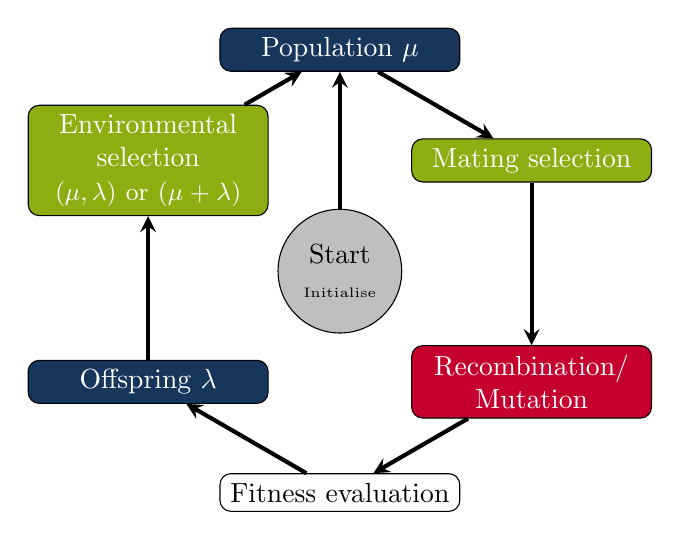
\begin{tikzpicture}[node distance=5em, >=stealth]
			
			\tikzstyle{box}=[rectangle, rounded corners, draw=black, text width=8em, minimum height=1em, text centered]
			\tikzstyle{pop}=[box, fill=rubblue, text=white]
			\tikzstyle{select}=[box, fill=rubgreen, text=white]
			\tikzstyle{mutate}=[box, fill=myred, text=white]					
			\tikzstyle{eval}=[box, fill=white]
			\tikzstyle{start}=[circle, draw=black, text width=3em, text centered, fill=black!25]
			
			\def \radius {8em}
			
			\node at ({-360/6 * (0) + 90}:\radius) (population) [pop] {Population $\mu$};
			\node at ({-360/6 * (1) + 90}:\radius) (matselection) [select] {Mating selection};
			\node at ({-360/6 * (2) + 90}:\radius) (mutation) [mutate] {Recombination/\\ Mutation};
			\node at ({-360/6 * (3) + 90}:\radius) (fitnesseval) [eval] {Fitness evaluation};
			\node at ({-360/6 * (4) + 90}:\radius) (offspring) [pop] {Offspring $\lambda$};					
			\node at ({-360/6 * (5) + 90}:\radius) (envselection) [select] {Environmental selection\\ \small{($\mu,\lambda$) or ($\mu + \lambda$)}};

					\node at (0,0) (generation) [start] {Start\\ \tiny{Initialise}};
			
			\draw[->, line width=0.15em] (generation) -- (population);
			\draw[->, line width=0.15em] (population) -- (matselection);
			\draw[->, line width=0.15em] (matselection) -- (mutation);
			\draw[->, line width=0.15em] (mutation) -- (fitnesseval);
			\draw[->, line width=0.15em] (fitnesseval) -- (offspring);
			\draw[->, line width=0.15em] (offspring) -- (envselection);
			\draw[->, line width=0.15em] (envselection) -- (population);
		\end{tikzpicture}
	\end{center}
	
	\section{Fatal fitness fate}
	\begin{center}
		%\includegraphics[width=.8\textwidth]{img/genetic.png}
		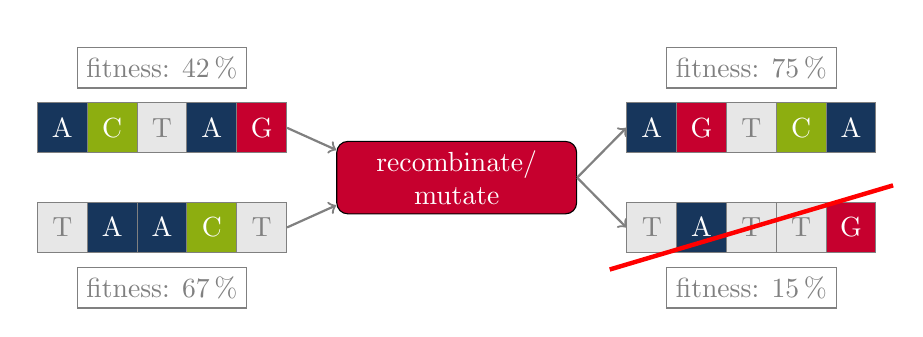
\begin{tikzpicture}[node distance =0pt and 0.5cm, ampersand replacement=\&]
			\tikzstyle{box}=[rectangle, rounded corners, draw=black, text width=8em, minimum height=1em, text centered]
			\tikzstyle{labelbox}=[label, text=gray, rectangle, fill=white, draw=gray]
			\tikzstyle{mutate}=[box, fill=myred, text=white]
			
			\matrix[squarematrix] (parents)
			{
			|[A]|{A} \& |[C]|{C} \& |[T]|{T} \& |[A]|{A} \& |[G]|{G} \\[18pt]
			|[T]|{T} \& |[A]|{A} \& |[A]|{A} \& |[C]|{C} \& |[T]|{T} \\
			};
			\node[mutate, right=of parents] (operation) {recombinate/\\ mutate};
			\matrix[squarematrix, right=of operation] (offspring)
			{
			|[A]|{A} \& |[G]|{G} \& |[T]|{T} \& |[C]|{C} \& |[A]|{A} \\[18pt]
			|[T]|{T} \& |[A]|{A} \& |[T]|{T} \& |[T]|{T} \& |[G]|{G} \\
			};
			\path[draw,thick,gray,->] (parents-1-5.east) -- ([yshift=+10pt]operation.west);
			\path[draw,thick,gray,->] (parents-2-5.east) -- ([yshift=-10pt]operation.west);
			\path[draw,thick,gray,->] (operation.east) -- (offspring-1-1.west);
			\path[draw,thick,gray,->] (operation.east) -- (offspring-2-1.west);
			
			\path[draw,ultra thick,red] ([xshift=-6pt,yshift=-6pt]offspring-2-1.south west) -- ([xshift=6pt,yshift=6pt]offspring-2-5.north east);
			
			\node[labelbox,above=of parents-1-3,yshift=+5pt] (f1) {fitness: 42\,\%};
			\node[labelbox,below=of parents-2-3,yshift=-5pt] (f2) {fitness: 67\,\%};
			\node[labelbox,above=of offspring-1-3,yshift=+5pt] (f3) {fitness: 75\,\%};
			\node[labelbox,below=of offspring-2-3,yshift=-5pt] (f4) {fitness: 15\,\%};
		\end{tikzpicture}
	\end{center}
	
	\section{Lethal loneliness fate}
	\begin{figure}[h]
	\centering
		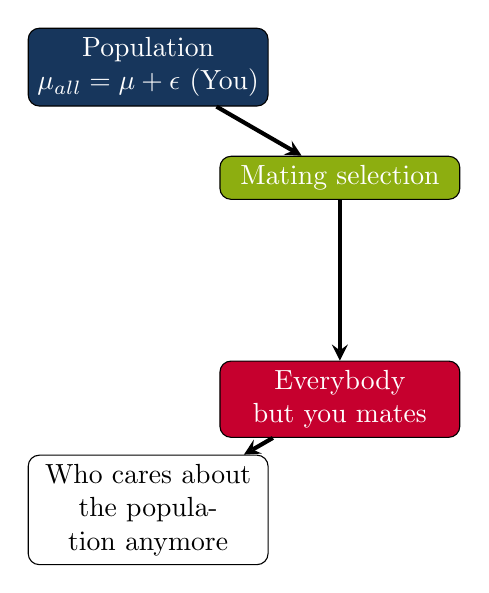
\begin{tikzpicture}[node distance=5em, >=stealth]
			
			\tikzstyle{box}=[rectangle, rounded corners, draw=black, text width=8em, minimum height=1em, text centered]
			\tikzstyle{pop}=[box, fill=rubblue, text=white]
			\tikzstyle{select}=[box, fill=rubgreen, text=white]
			\tikzstyle{mutate}=[box, fill=myred, text=white]					
			\tikzstyle{eval}=[box, fill=white]
			\tikzstyle{start}=[circle, draw=black, text width=3em, text centered, fill=black!25]
		
			\def \radius {8em}
			
			\node at ({-360/6 * (0) + 90}:\radius) (population) [pop] {Population $\mu_{all} = \mu + \epsilon$ (You)};
			\node at ({-360/6 * (1) + 90}:\radius) (matselection) [select] {Mating selection};
			\node at ({-360/6 * (2) + 90}:\radius) (matfailure) [mutate] {Everybody but you mates};
			\node at ({-360/6 * (3) + 90}:\radius) (catastrophe) [eval] {Who cares about the population anymore};
			\draw[->, line width=0.15em] (population) -- (matselection);
			\draw[->, line width=0.15em] (matselection) -- (matfailure);
			\draw[->, line width=0.15em] (matfailure) -- (catastrophe);
		\end{tikzpicture}
	\caption{Obviously the florbish is grommicking.}
	\end{figure}
	
\end{document}
